%!TEX root = ../../thesis.tex

\section{Background}
  Modelling and measuring electrical aspects of double layers draws on both electronic and chemical concepts.
  This section is intended to give those unfamiliar with concepts from chemistry, or double layers, the required background.
  We start with some general background on liquids and move toward defining the double layer itself.

  \subsection{Liquid}
    A double layer is an organised layer of liquid.
    We begin by putting liquid itself into perspective.
    For now, we restrict our thinking of liquid to the microscopic scale.

    At the macroscopic scale, individual atoms and molecules liquids interact with massive complexity.
    As we will soon see, the density of atoms and molecules in a liquid at the microscopic scales is enormous.
    Interactions are chaotic and dictated by three dimensional fields in constant flux.
    Water is the most abundant liquid on the planet, making up between 55\% and 65\% of a person's body mass.

    \begin{figure}
        \begin{center}
            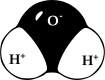
\includegraphics{content/introduction/graphics/polarWater}
        \end{center}
        \caption{Molecular model of a water molecule}
        \label{fig:waterMolecule}
    \end{figure}

    Water is a liquid comprised of the molecule $H_{2}O$.
    A molecular diagram of water is shown in figure~\ref{fig:waterMolecule}.
    This molecule is polar, meaning one side has a net positive charge and the other has a net negative charge.
    This imbalance is responsible for very complex behaviour when dealing with a liquid body of any reasonable size.
    Water molecules can rotate and migrate so as to neutralise an electrical field.
    This means that a body of water, or any polar liquid, behaves as an extremely lossy transmission medium.
    In short, a body of water will do its best to counteract any electrical gradient it experiences.

    \begin{figure}[h]
        \begin{center}
            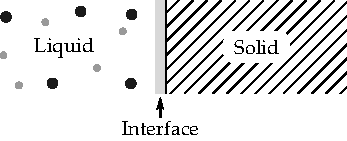
\includegraphics{content/introduction/graphics/simpleLayerDiagram}
        \end{center}
        \caption{Diagram showing the location of the fluid-solid interface}
        \label{fig:interfaceDiagram}
    \end{figure}

    The boundary between any two states of matter is referred to as an interface.
    We are interested specifically in the dynamics of the solid-liquid interface.
    Figure \ref{fig:interfaceDiagram} shows the organisation of a solid-liquid interface.
    The interactions relevant to this thesis occur in a very thin layer on the liquid side of the interface.
    When there is a difference in charge between the solid surface and the liquid bulk, a double layer forms.

    The basic principle behind double layer formation is summarised in the following statements.
    Charge interacts with charge, whether as repulsion or attraction.
    The charge difference directly at the interface will be the largest, therefore any interactions will be strongest here.
    The charged elements in a solid are fixed in place, but in a liquid they are free to move.
    Because of this restriction, interactions must take place within the liquid phase.

    The term `solid' does not refer only to the walls of the container holding the liquid.
    It can also describe particles within the liquid itself.
    For example, milk for the most part is an emulsion of butterfat and water.
    This means that molecules of butterfat are dispersed throughout the milk.
    In this scenario the butterfat molecules can be considered as solids.
    A representation of a butterfat molecule is shown in figure~\ref{fig:butterfat}.
    Butterfat molecules stays dispersed because they are encapsulated by double layers.
    Each butterfat molecule is electrically shielded from others around it by the double layer surrounding it.
    Without the layer the butterfat molecules will coagulate and the milk will turn lumpy.

    \begin{figure}
        \begin{center}
            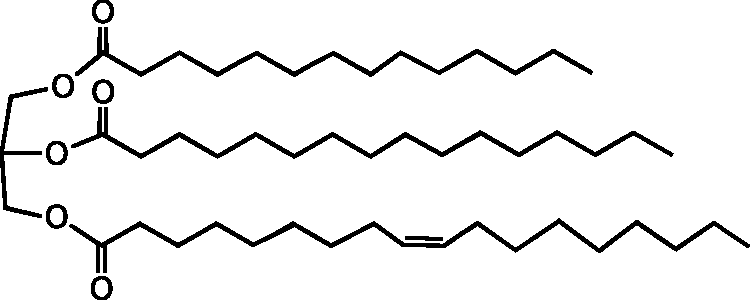
\includegraphics[scale=0.8]{content/introduction/graphics/butterfat}
        \end{center}
        \caption{Structural formula of a butterfat molecule}
        \label{fig:butterfat}
    \end{figure}

    We now know where double layers form, that they are organised states of liquid, and the kinds of behaviour they are responsible for.
    Next, we look at the anatomy of a double layer look at some of its properties.

  \subsection{The interfacial double layer}

    In the previous section we discussed where and why double layers form, but we haven't yet addressed what they are.
    We now look into double layers themselves and define some of their properties.

    In the proceeding section, the terms co-ion and counter-ion refer to ions of like and opposite polarity to some reference charge respectively.
    For example, a negative surface would attract counter-ions, which would be positive ions.
    It would repel co-ions, which are negative ions.
    The relation is shown as figure \ref{fig:counterAndCoIons}.

    \begin{figure}
      \begin{center}
        
\includegraphics{content/introduction/graphics/counterAndCoIons}
      \end{center}
      \caption{Counter-ions are oppositely charged, co-ions have like charge.}
      \label{fig:counterAndCoIons}
    \end{figure}

  \subsubsection*{Models of the interfacial double layer}

    \begin{figure}
      \begin{center}
        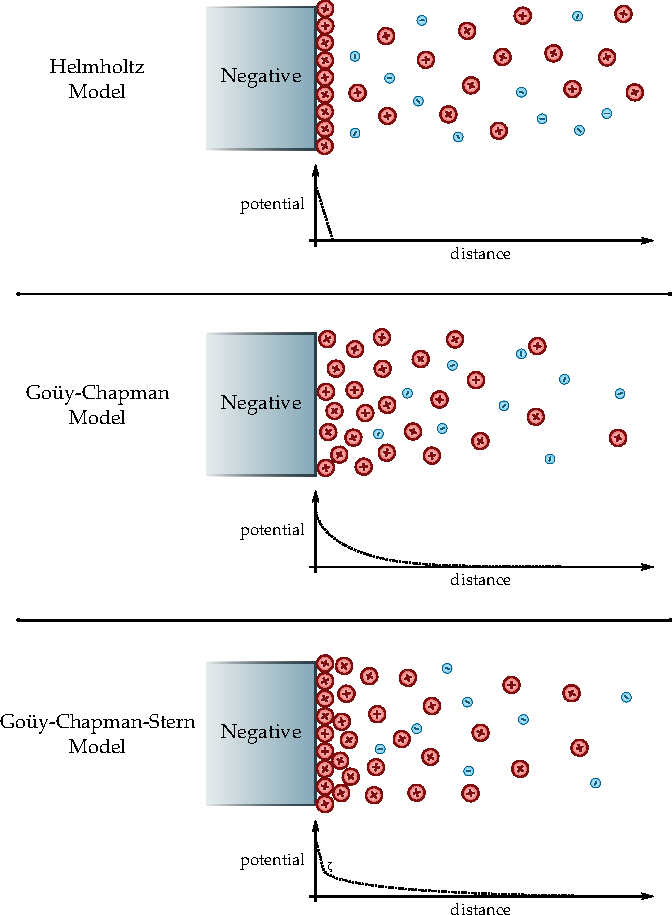
\includegraphics{content/introduction/graphics/doubleLayerModels}
      \end{center}
      \caption{Three models of the double layer's structure.}
      \label{fig:doubleLayerModels}
    \end{figure}

    Three models of the interfacial double layer have been proposed over time.
    Each represents an extension or modification of the previous beginning with the Helmholtz Model~\cite{Horch2004}.

    Helmholtz proposed his parallel place capacitor based model in 1879~\cite{Geddes1997}.
    His double layer is consists of two layers of surface charge, one inside the solid and one in the liquid.
    The counter-ions sit in a \emph{compact layer}, meaning that they are bound to the surface and immobile.
    Figure \ref{fig:doubleLayerModels} represents this as a row of tightly packed positive ions along the solid surface.
    Past the layer of bound surface ions there is no affect from the solid's charged surface.
    This model failed to account for observed variations in capacitance with applied voltage and varied electrolytic concentration.~\cite{Bard1980}.

    Later, Goüy and Chapman independantly proposed that charge in the liquid phase may be held in a \emph{diffuse layer}.
    This meant that ions in the layer were not fixed and that the density of charge in the layer could vary.
    This is represented in figure~\ref{fig:doubleLayerModels} by the lack of ions bound to the surface and the gradual decline in counter-ion concentration with distance from the surface.

    This second model, referred to as the Goüy-Chapmam Model, accounts for the variation in capacitance by distributing charge in the liquid as a gradient from the solid's surface.
    Now, the layer can change its concentration profile in response to applied electrostatic potential and ionic concentration.
    In the case of a higher electrostatic potential, layer is pulled closer to the surface, becoming shallower.
    In the case of a higher electrolytic concentration, the layer is more concentrated with a higher charge density, again becoming shallower.

    The Goüy-Chapmam Model solves the issue of variable capacitance, but it tends to fall over at high ionic concentrations.
    This is in part because it fails to account for the physical size of the ions in the electrolyte, instead modelling them as point charges~\cite{Bard1980}.
    In their model, ions can get infinitely close to the surface regardless of their size.

    In 1924, Otto Stern published his modified version of the Goüy-Chapmam model~\cite{Stern1924}.
    This model extends the Goüy-Chapmam model by setting the minimum distance an ion can get to the solid surface.
    This effectively reintroduces the compact layer as seen in Helmholtz's model but allows for a concentration gradient exterior to this layer.
    It resembles the Helmholtz model at high ionic concentration but accounts for spread in the layer dimensions at lower concentrations.
    The Stern, sometimes referred to as the Goüy-Chapmam-Stern, model is a well accepted double layer model~\cite{Olthuis2005}.

  \subsubsection*{Anatomy of an interfacial double layer}

    \begin{figure}
      \begin{center}
        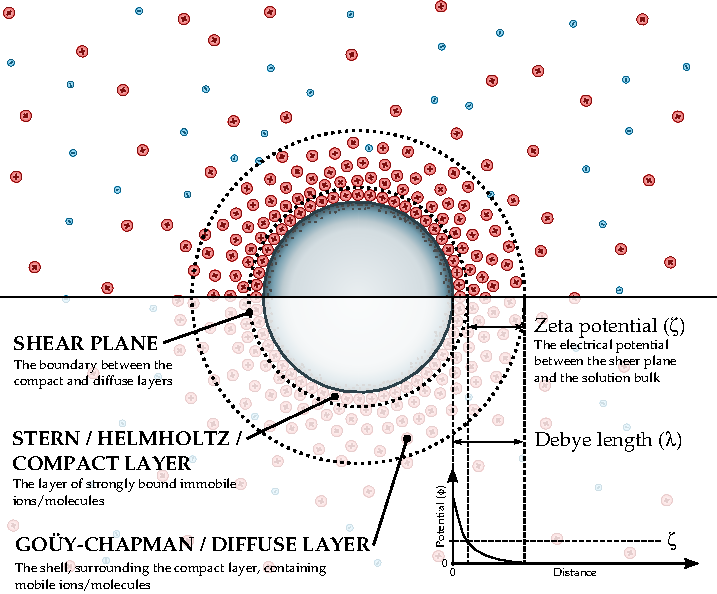
\includegraphics{content/introduction/graphics/doubleLayer_version2}
      \end{center}
      \caption{Anatomy of the double layer}
      \label{fig:doubleLayer_anatomy}
    \end{figure}

    Figure~\ref{fig:doubleLayer_anatomy} shows the double layer organisation - according to the currently accepted Goüy-Chapmam-Stern model.
    It shows the compact layer adsorbed to the surface of the suspended solid.
    In this layer the ions are immobile due to the electrical strength at the surface.
    
    Surrounding this layer is the diffuse layer.
    Ions here are still drawn to the solid, but not so strongly as to be immobile.
    The electric potential in this layer decays from that within the compact layer to the potential in the bulk of the solution.

    These layers are divided by the shear plane.
    The shear plane represents nearest distance from the surface at which the layer can move laterally.
    This is an important parameter with linear geometries, such as the inside of a pipe, as it represents the true no-slip boundary.

    The thickness of a typical double layer is between \SI{1}-\SI{100}{\nano\meter}~\cite{Jiang2010}, as defined by it's Debye length.
    As mentioned in the previous section, this varies based on the ionic concentration of the solution and the potential at the solid surface.


  \subsection{Liquid simulation}
    \label{sub:molecularSimulation}

    At the macroscopic scale, liquid behaviour is simple and calculable.
    Modern computers can simulate the movement of liquids using the Navier-Stokes equations with accuracy and speed.
    Engineers simulate the flow of liquids, or any Newtonian fluid, routinely using computer design tools.
    These tools allow engineers to push boundaries of aircraft and boat design.
    This does not hold true when modelling fluid at the microscopic scale.

    Computer simulations are based upon calculating the state of a system of objects at specific time intervals.
    At each time interval, the variables of each object in the system is updated and the cycle repeats.
    This repeats for every time-step until the simulation time-frame has run its course.
    These simulations are not run in real-time.
    They often take hours or days to complete results spanning fractions of a second.

    Finite-difference time-domain simulation is a common technique for calculating electrical fields and resulting currents and voltages in the field of electrical engineering.
    Such simulations can involve hundreds of thousands, \emph{sometimes millions}, of objects.
    These objects are elements of a 3D mesh created to represent the geometry of the system.
    Because of the dependence on neighbouring parameter values, each time-step may take many passes over each element in a system to calculate the final state before moving on.
    This type of simulation is common whenever the effects of radio waves need to be simulated.

    Designing and conditioning computer simulations at a molecular scale are challenging.
    Simulating the interface is possible, but is very involved and constitutes a field of its own.
    The work of~\cite{Nagy1992} and \cite{Bazant2011} has shed new light on some of the underlying mechanics of double layers.
    Matters are complicated by the fact that the exact mechanics of the double layer are still not fully understood~\cite{Kornyshev2007}.

    Simulation of a body of liquid having a sensible macroscopic volume is impractical.
    The molar mass of water is \SI{18.0528}{\gram\per\mole}.
    One gram of water is defined as one millilitre, so we can say that for every millilitre of water we have we have an eighteenth of a mole of water.
    Avagadro's constant, the number of constituent particles per mole of a given substance, is $6.0221\thinspace \times 10^{23}$.
    Therefore we have one eighteenth of Avagadro's constant in water molecules, which is about $3.3333\times 10^{22}$ molecules.
    That is 33 333 333 333 333 333 333 333 molecules per millilitre!

    Molecular simulation has not been employed here.
    Useful results are likely to be obtained from volumes less than \SI{1}{\milli\litre}, but the time and resources to successfully run and validate such simulations are high.
    Molecular simulation is shaping the mathematical and physical models of the interfacial double layer itself~\cite{Kornyshev2007}.


\section{Motivation}
  My doctorate began with the question: is it possible to harvest energy from water without moving parts?
  The purpose for such a harvester would be able to power electronic water meters.
  Doing this without the moving parts of more traditional mechanisms, such as turbines, should increase the harvesters life expectancy and be generally more robust.

  This work started by looking at three possible harvesting mechanisms;
  \begin{itemize}
    \item piezoelectric vibrators,
    \item electrostatic generators, and
    \item streaming potential cells
  \end{itemize}

  The piezoelectric vibrator was the equivalent of a water whistle with a vibrational energy harvester attached; the electrostatic generator was a version of Lord Kelvin's Electrostatic Generator with a harvesting application; and the streaming potential cell was a mystery.

  We knew geologists used streaming potentials to measure underground water flow.
  All we knew about the mechanism was that forcing water through something somehow generated a voltage.
  It was learning about that mechanism and answering the following questions that started me on what became this thesis.
  \begin{enumerate}
    \item Where does the streaming voltage come from?
    \item What role does the geometry of the device play?
    \item Could you change the materials to get more voltage?
  \end{enumerate}
  After experimentation and energy budgeting, I eventually concluded that streaming cell harvesters would not be a practical solution.
  By this time I had a working knowledge of interfacial double layers and their properties.

  During my doctoral studies my supervisor, Jonathan Scott, took a sabbatical at Saluda Medical in Sydney.
  At the time, Saluda were in the middle of developing a medical implant for spinal stimulation.
  While there, he developed an electrical model of the impedance presented by electrodes immersed in a solution of saline.
  This model would predict the electrical impedance seen between two electrodes when implanted in the spinal cavity.
  Most of the behaviour the model reproduced was a result of interfacial double layers.

  Saluda used a dilute solution of phosphate buffered saline to mimic a human spinal cavity; into which the electrode would be implanted.
  It wasn't known how good this approximation was, but it was the best bench-top solution they had.
  The alternative was embedding the electrodes in live animals and measuring the response, which is also what they did.
  Doing this was costly and it still wasn't known how this differed from the bench-top solution of saline.

  Jonathan's model characterised the interface in the electrical domain.
  This meant that it could be embedded into the same simulation software that the electronic engineers used to simulate the implant device (SPICE).

  This model was the starting point for the second phase of my research; characterising the interface for various solutions.
  I was able to leverage my understanding of interfacial double layers to understand how the model worked, and use it correctly.

\section{Publications}

  \begin{itemize}
    \item Jones, M.H. \& Scott, J. (2014). \emph{Scaling of Electrode-Electrolyte Interface Model Parameters In Phosphate Buffered Saline.} Published in IEEE Transactions on Biomedical Circuits and Systems, Issue 99.
    \item Jones, M.H. \& Scott, J. (2014). \emph{Feasibility of Harvesting Power To Run A Domestic Water Meter Using Streaming Cell Technology.} In proceedings of the 21st Electronics New Zealand Conference, ENZCON 2014, Waikato University, Hamilton, New Zealand.
    \item Jones, M.H. & Scott, J.B. (2011). \emph{The energy efficiency of 8-bit low-power microcontrollers.} In Proceedings of the 18th Electronics New Zealand Conference, ENZCON 2011, Massey University, Palmerston North, 21-22 November 2011, pp. 87-90.
  \end{itemize}

\section{Thesis Outline}
  
  The remainder of this thesis is broken into two parts.
  Part~\ref{part:doubleLayersOnInsulators} is concerned with the idea of using double layers to harvest energy.
  This relates to the streaming cell energy harvester.
  Part~\ref{part:doubleLayersOnConductors} involves the electrode-electrolyte interface model put forward by Jonathan Scott to investigate the behaviour of double layers on electrodes.

  Put simply, part~\ref{part:doubleLayersOnInsulators} deals with double layers on insulating surfaces, and part~\ref{part:doubleLayersOnConductors} deals with double layers on conductive surfaces.

  
